\section{L5}


\subsection{Basics}


\paragraph{Scenario}

Sender S 和 receiver R 彼此有有一把相同的 key \(k\),且 S 想要發送訊息給 R。 \\
在發送訊息前,S 會先使用 \(k\) 將明文 \(m\) 加密為密文 \(c\)(\(c \leftarrow \Enc_k(m)\)),之後 S 將 \(c\) 傳送給 R。 \\
R 在收到 \(c\) 後,使用同一把 key \(k\) 將 \(c\) 解密(\(m \coloneq \Dec_k(c)\))來得到 \(m\)。

關於這個 scenario 的正式的定義可以參見 Definition \fullref{def:priv_key_enc}。


\paragraph{安全性定義}

使用前面提到的 \(PrivK_{A, \Pi}^{eav}\),參見 \fullref{PrivK}。


\subsection{EAV-security}

EAV = eavesdropping

\begin{definition}[EAV-secruity of private key encryption]
	A private key encryption scheme \(\Pi\) is \textbf{EAV-secure} if for all PPT adversary \(A\), there is a negligible function \(\negl\) such that for all \(n\),
	\[\Pr[PrivK_{A, \Pi}^{eav}(n) = 1] \leq \frac{1}{2} + \negl(n)\]
	(The probability is taken over randomness used by adversary and used in experiment.)
\end{definition}


\paragraph{Equivalent Formulation of EAV-security}

前一節 EAV-security 的定義等價於下面這句話: \\
「無論 PPT adversary \(A\) 看到由 \(m_0\) 或 \(m_1\) 加密過後的密文,其表現都相同。」 \\
(Every PPT adversary behaves the same whether it sees ciphertext of \(m_0\) or \(m_1\).)

更精確的定義是:
\begin{myItemize}
	\item 修改之前的定義為 \(PrivK_{A, \Pi}^{eav}(n, b)\),其定義都和之前一樣,除了 \(b\) 是固定的,而不是隨機選擇的。
	\item 定義 \(out_A(PrivK_{A, \Pi}^{eav}(n, b)) = b'\),其中 \(b'\) 是 \(A\) 的 output。
	\item 沒有 PPT adversary \(A\) 可以知道現在是 experiment \(PrivK_{A, \Pi}^{eav}(n, b)\) 或 \(PrivK_{A, \Pi}^{eav}(n, b)\)。
\end{myItemize}

正式定義如下:
\begin{definition}[equivalent formulation of EAV-security]
	\(\Pi\) is EAV-secure if for all PPT adversary \(A\), there is a negligible function \(\negl\) such that
	\[ | \Pr[out_A(PrivK_{A, \Pi}^{eav}(n, 0)) = 1] -
		 \Pr[out_A(PrivK_{A, \Pi}^{eav}(n,1)) = 1] \leq \negl(n)\]
\end{definition}

\begin{center}
	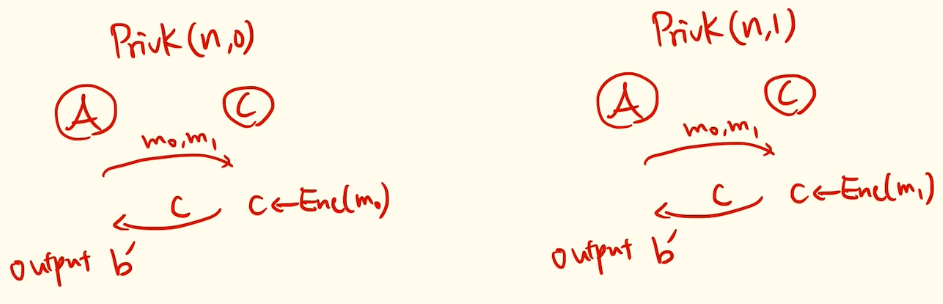
\includegraphics[width=0.8\textwidth, keepaspectratio]{equivalent _of_private_key_encryption.png}
\end{center}

\subparagraph{Quiz}

In \(PrivK\), we define \(A\) to choose two messages with the same length. \\
Please write your thought for the impossibility to support arbitrary-length messages.


\subsection{Private Key Encryption}


\paragraph{Pseudorandom Generator}

\begin{definition}[pseduorandom generator, PRG]
	Let \(l\) be a polynomial and \(G\) is a deterministic polynomial-time algorithm. For any \(n\) and input \(s \in \{0, 1\}^n\), the output of \(G(s)\) is \(l(n)\)-length. \\
	We say \(G\) is a PRG if:
	\begin{myItemize}
		\item Exapnsion: for every \(n\), it holds \(l(n) > n\). \(l\) is a so-called expansion factor of \(G\).
		\item Pseudorandomness: for any PPT algorithm \(D\) (aka distinguisher), there is a negligible function \(\negl\) such that
		\[ | \Pr[D(G(s)) = 1] - \Pr[D(r) = 1] | \ \leq \ \negl(n)\]
		where \(s \in \{0, 1\}^n\) and \(r \in \{0, 1\}^{l(n)}\) is a turly random variable.
	\end{myItemize}
\end{definition}


\paragraph{PRG-based Construction of Fixed-length Private Key Encryption}

Let \(G\) be a PRG with expansion factor \(l\). \\
Scheme \(\Pi = \Gen, \Enc, \Dec\).
\begin{myItemize}
	\item \(\Gen(1^n)\): on input \(1^n\), choose uniform \(k \in \{0, 1\}^n\).
	\item \(\Enc(k, m)\): with input of a message \(m \in \{0, 1\}^{l(n)}\) and outputs a ciphertext \(c = G(k) \oplus m\)
	\item \(\Dec(k, c)\): with input of a ciphertext \(c \in \{0, 1\}^{l(n)}\) and outputs a message \(m = G(k) \oplus c\)
\end{myItemize}

這種構造法和 OTP(見 \fullref{def:OTP})很像。那時候的 OTP 會遇到 pefect secrecy 的限制,也就是 key 的長度至少要和 message 一樣長(\(|\K| \geq |\M|\))。在這裡,我們通過 PRG 來將原本的 key 長度 \(n\) 擴展成 \(l(n)\),藉此來降低 key 的長度。而其代價就是,這種使用 PRG 的方法一定不是 perfect secrecy。

P.S. 由於 private key encryption 要求雙方要事先使用安全通道交換同一把 key。若在這種情景下使用和 message 一樣長的 key,那我們就可以直接使用這個安全通道交換訊息本身了,而無需進行加密。


\paragraph{PRG-based construction is EAV-secure}

\begin{theorem}
	If \(G\) is a pseudorandom generator, then the construction \(\Pi\) is a EAV-secure.
\end{theorem}

其逆否命題為「如果 \(\Pi\) 不是 EAV-secure,則 \(G\) 也不是 PRG」。

\subparagraph{證明思路}

由 \(D\) 扮演 challenger。 \\
在 reduction 時是 \(D\) 包在 \(A\) 的外面。

\begin{figure}
	\subfloat[Distinguisher \(D\) and adversary \(A\)]{
		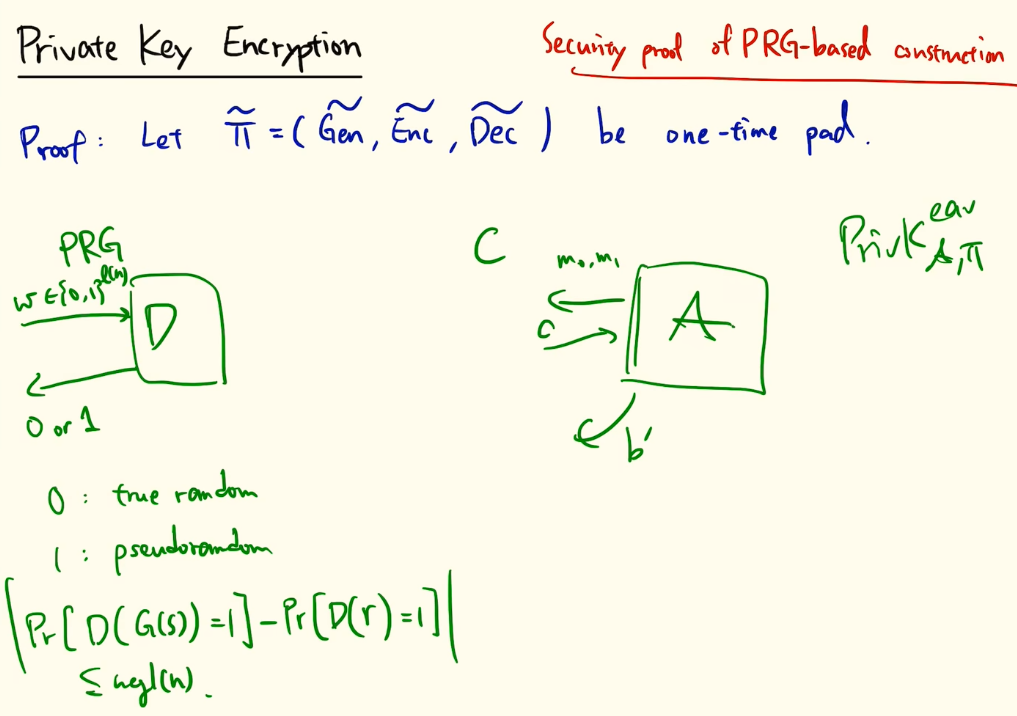
\includegraphics[width=0.6\textwidth, keepaspectratio]{proof_of_PRG-based_construction_1.png}
	}
	\subfloat[Reduction in proof]{
		\label{fig:reduction}
		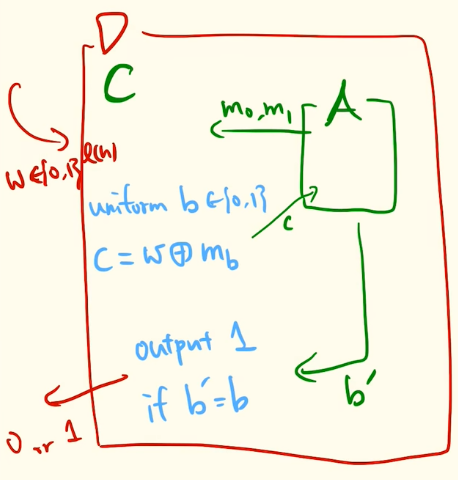
\includegraphics[width=0.4\textwidth, keepaspectratio]{proof_of_PRG-based_construction_2.png}
	}
\end{figure}

Let \(\widetilde{\Pi} = (\widetilde{\Gen}, \widetilde{\Enc}, \widetilde{\Dec})\) be one-time pad.

\begin{enumerate}[itemsep=10pt]
	\item If \(w\) is uniform chosen form \(\{0, 1\}^{l(n)}\),		
		\begingroup
		\setlength{\fboxsep}{1pt}
		\[ \Pr[D(w) = 1] = \Pr[PrivK_{A, \colorbox{yellow}{\scalebox{0.6}{\(\widetilde{\Pi}\)}}}^{eav}(n) = 1]
							= \frac{1}{2}\]
		\endgroup
		
		這種情況是 one-time pad 的情況,也就是使用 true randomness。
		
	\item If \(w = G(k)\) by choosing uniform \(k \in \{0, 1\}^n\),
		\begingroup
		\setlength{\fboxsep}{1pt}
		\[ \Pr[D(G(k)) = 1] = \Pr[PrivK_{A, 
		\colorbox{yellow}{\scalebox{0.6}{\(\Pi\)}}}^{eav}(n) = 1]\]
		\endgroup
		
		這種情況是使用 pseudorandomness。 \\
		這個機率是我們所要證明的,可以透過第三點來反推其機率為 \(\leq \displaystyle\frac{1}{2} + \negl(n)\)
		
	\item If \(G\) is PRG,
		\[ | \Pr[D(G(k)) = 1] - \Pr[D(w) = 1] | \ \leq \ \negl(n)\]
\end{enumerate}

\subparagraph{Proof details}

Let \(A\) be a PPT adversary. Our goal is to contract a distinguisher \(D\) (which is going to break PRG) that takes a string \(w\) as input.

Goal of \(D\): determine whether
\begin{myEnumerate}[label=(\roman*)]
	\item \(w\) was chosen uniformly (where \(w \in \{0, 1\}^{l(n)}\))
	\item \(w\) was generated by choosing uniform \(k \in \{0, 1\}^n\) and computing \(w = G(k)\) (where \(w \in \{0, 1\}^{l(n)}\) and \(l(n) > n\))
\end{myEnumerate}

Output of \(D\): outputs 1 if case (i) mentioned above; otherwise, outputs 0

Theorem used:
\[ | \Pr[D(r) = 1] - \Pr[D(G(k)) = 1] | \ \leq \ \negl(n)\]
where \(r \leftarrow \{0, 1\}^{l(n)}\), and \(k \leftarrow \{0, 1\}^n\).

Activites of \(D\): (connect \(A\) and \(D\)) \\
Emulate the eav experiment \(PrivK_{A, \Pi}^{eav}\) for \(A\)
\begin{myItemize}[label=—]
	\item If \(A\) wins, \(D\) thinks \(w \coloneq G(k)\).
	\item If \(A\) fails, \(D\) thinks \(w\) is uniform chosen.
\end{myItemize}

\begin{myProof}
	(Refer to figure \hyperref[fig:reduction]{Reduction in proof}) \\
	Distinguisher \(D\) get an input of a string \(w \in \{0, 1\}^{l(n)}\).
	\begin{steps}
		\item Run \(A\) to obtain a pair of messages \(m_0, m_1 \in \{0, 1\}^{l(n)}\)
		\item Choose a uniform bit \(b \in {0, 1}\). Set \(c = w \oplus m_b\)
		\item Send \(c\) to \(A\)
		\item Later, \(A\) returns \(b'\)
	\end{steps}
	
	\(D\) outputs
	\begin{myItemize}[label=—]
		\item 1, if \(b' = b\)
		\item 0, if \(b' \neq b\)
	\end{myItemize}
	
	Note that probability of output of \(D\) is related to \(\Pr[PrivK_{A, \Pi}^{eav}]\). \\
	If \(\displaystyle \Pr[PrivK_{A, \Pi}^{eav}] > \frac{1}{2} + \negl\),
	\begin{align*}
		\Pr[out_D = 1] > \frac{1}{2} + \negl \\
		\Pr[out_D = 0] \leq \frac{1}{2} - \negl
	\end{align*}
\end{myProof}


\subsection{Chosen Plaintext attack \& CPA-security}

CPA = Chosen Plaintext Attack


\paragraph{CPA security}

在這個情景下的 adversary \(A\) 可以存取 encryption oracle。

Encryption oracle:是一個黑盒子,我們不知道其運作原理,但給它輸入和取得它的輸出。\(A\) 可以將明文 \(m\) 給 oracle,之後 oracle 會將明文加密為密文 \(c \leftarrow \Enc_k(m)\) 回傳給 \(A\)。

\subparagraph{Experiment \quad \(PrivK_{A, \Pi}^{cpa}\)}

\begin{steps}
	\item \(A\) 可以選擇明文 \(m_i\) 給 \(C\)
	\item \(C\) 建立密鑰 \(k \leftarrow \Gen(1^n)\),並將明文加密為密文 \(c_i \leftarrow \Enc(m_i)\) 回傳給 \(A\)。
	\item \(A\) 此時可以將這些收集到明文-密文對(plaintext-ciphertext pair)儲存起來。由於 \(A\) 是 PPT adversary,所以 \(A\) 可以收集的 pair 數為 poly-many。
	\item \(A\) 選擇 \(m_0\) 和 \(m_1\) 傳給 \(C\) 進行 chanllenge。之後的事情都和之前的 EAV-secure 的 experiment 一樣。
	\item 若 \(A\) 贏了,則 \(PrivK_{A, \Pi}^{cpa}(1^n) = 1\)。
\end{steps}

P.S. 前三步稱為 encryption oracle query。而 challenge 之後一樣可以進行 eneryption oracle query,直到 \(A\) output \(b'\)。

\subparagraph{Quiz}

Show PRG-based construction \(\Pi\) is not CPA-secure. \\
(Hint: give \(A\) in \(PrivK_{A, \Pi}^{\colorbox{yellow}{\scalebox{0.7}{\(cpa\)}}}\) to break \(\Pi\))

